\documentclass[10pt]{article}
\usepackage[polish]{babel}
\usepackage[utf8]{inputenc}
\usepackage[T1]{fontenc}
\usepackage{amsmath}
\usepackage{amsfonts}
\usepackage{amssymb}
\usepackage[version=4]{mhchem}
\usepackage{stmaryrd}
\usepackage{graphicx}
\usepackage[export]{adjustbox}
\graphicspath{ {./images/} }

\title{LIGA MATEMATYCZNA \\
 PAŹDZIERNIK 2009 \\
 SZKOŁA PODSTAWOWA }

\author{}
\date{}


\begin{document}
\maketitle
\section*{ZADANIE 1.}
Ania zgubiła sześcienną kostkę do gry i samodzielnie wykonała inną kostkę w taki sposób, że sumy oczek na parach ścianek przeciwległych tworzą trzy kolejne liczby naturalne (w typowej kostce do gry sumy oczek na ściankach przeciwległych są równe). Okazało się, że suma oczek na pewnych trzech ściankach mających wspólny wierzchołek jest równa 14. Ile oczek jest na ściance przeciwległej do ścianki z trzema oczkami?

\section*{ZADANIE 2.}
Czy z jedenastu kwadratów o bokach \(1 \mathrm{~cm}, 1 \mathrm{~cm}, 2 \mathrm{~cm}, 2 \mathrm{~cm}, 2 \mathrm{~cm}, 3 \mathrm{~cm}, 3 \mathrm{~cm}, 4 \mathrm{~cm}, 6 \mathrm{~cm}\), \(6 \mathrm{~cm}, 7 \mathrm{~cm}\) można zbudować kwadrat?

\section*{ZADANIE 3.}
Dwóch uczniów rozwiązuje dwa rebusy w ciągu dwóch minut. Ile rebusów rozwiąże 10 uczniów w ciągu 10 minut?

\section*{ZADANIE 4.}
Piszemy liczbę 0 , następnie liczbę 1 i znowu 1, potem piszemy najmniejszą z tych liczb całkowitych nieujemnych, która nie wystąpiła na trzech poprzednich miejscach. Dalej postępujemy podobnie. Jaka liczba będzie na 99 miejscu?

\section*{ZADANIE 5.}
Obwody zamalowanych prostokątów są równe 24 cm i 12 cm . Oblicz obwód prostokąta \(A B C D\).\\
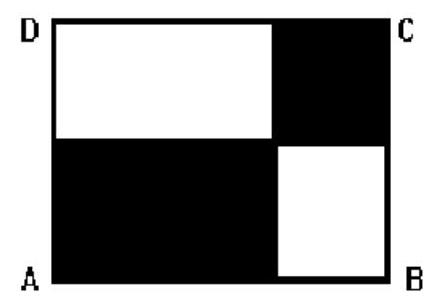
\includegraphics[max width=\textwidth, center]{2024_11_21_e15659a0efdc0a6e5618g-1}


\end{document}